\documentclass[tikz,border=0pt,convert={density=1000,size=2000x1000,outext=.png}]{standalone}
\usepackage{tikz}

\usetikzlibrary{backgrounds,arrows,shapes,shapes.misc,shapes.arrows,chains,matrix,positioning,scopes,decorations.pathmorphing,shadows, tikzmark}

\tikzset{
	state/.style={
		rectangle,
		rounded corners,
		draw=black, very thick,
		minimum height=2em,
		inner sep=2pt,
		text centered,
	},
}

\usepackage{amsmath,amssymb}

\usepackage{color}

\definecolor{light-gray}{gray}{0.9}
\begin{document}

\begin{footnotesize}

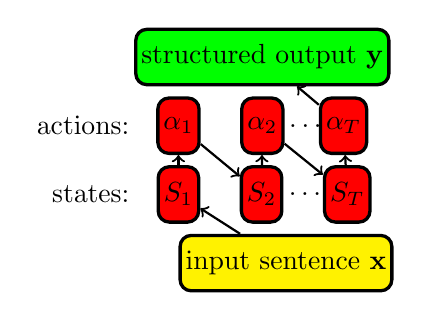
\begin{tikzpicture}[node distance=5mm]
\node	(input)	[state, fill=yellow]			{input sentence $\mathbf{x}$};
\node	(state1)				[state, fill=red]	[above=of input.west]	{$S_1$};
\node	(action1)				[state, fill=red]	[above=of state1.center]	{$\alpha_1$};
\node	(actions)				[left=of action1.center]	{actions:};
\node	(states)				[left=of state1.center]	{states:};
\node	(action2)				[state, fill=red]	[right=of action1]	{$\alpha_2$};
\node	(state2)				[state, fill=red]	[right=of state1]	{$S_2$};
\node	(actiont)		    	[right=of action2.west]	{$\ldots$};
\node	(actionT)				[state, fill=red]	[right=of actiont.west]	{$\alpha_T$};
\node	(statet)		    	[right=of state2.west]	{$\ldots$};
\node	(stateT)				[state, fill=red]	[right=of state2]	{$S_T$};
\node	(output)				[state, fill=green]	[above=of action2.center]	{structured output $\mathbf{y}$};


\path[thick, ->] (input) edge (state1);
\path[thick, ->] (state1) edge (action1);
\path[thick, ->] (action1) edge (state2);
\path[thick, ->] (state2) edge (action2);
\path[thick, ->] (action2) edge (stateT);
\path[thick, ->] (stateT) edge (actionT);
\path[thick, ->] (actionT) edge (output);


\end{tikzpicture}

	
\end{footnotesize}

\end{document}